
\section{Results} \label{sec:results}
Following the protocol outlined above, we evolved 100 networks for each of the seven variants of the model. For all networks, we set network size to 2000 nodes; $A = 1$; and $m = 1$. These choices are discussed in the appendix.

\subsection{Goodness-of-fit of the power-law model} \label{ssec:GOF of power law}

For each network evolved we computed two best-fit power-law models, one for $k>=1$ and the other for $k>=k_{min}$ where $k_{min}$ is the in-degree the minimizes the Kolmogorov-Smirnov distance between the fitted function and the data over $k>=k_{min}$. On each of these models, we ran a goodness-of-fit test as described in section 3.2. This resulted in two distributions of p-values for our control group, plus two more for each of our six treatment groups. Table \ref{table:GOF1}
 and \ref{table:AvgPvall} report descriptive statistics for these distributions.

\begin{table}[h]
\centering
\caption{Number of rejects (out of 100 runs) for goodness-of-fit tests of power-law models to in-degree distributions of interaction networks in online communities, with no onboarding (control group) and with onboarding. Power-law models are estimated over all nodes with degree $k>=1$}
\label{table:GOF1}
\begin{tabular}{lllllll}
\hline
\multicolumn{7}{c} {Control group: 23}\\
\hline
  & nu2 = 0.0 & nu2 = 0.2 & nu2 = 0.4 & nu2 = 0.6 & nu2 = 0.8 & nu2 = 1\\
nu1 = 0.0        & 83        & 81        & 83        & 88        & 82        & 85      \\
nu1 = 0.2          & 78        & 73        & 70        & 73        & 73        & 70      \\
nu1 = 0.4          & 66        & 65        & 61        & 69        & 76        & 56      \\
nu1 = 0.6          & 59        & 67        & 63        & 51        & 70        & 71      \\
nu1 = 0.8          & 55        & 60        & 66        & 61        & 60        & 61      \\
nu1 = 1            & 65        & 62        & 54        & 60        & 54        & 57   \\
\hline  
\end{tabular}
\end{table}


From Table \ref{table:GOF1}, we conclude that onboarding seems to have some effect on the goodness-of-fit of the generated data to their respective best-fit power-law models when formula. The effect goes in the direction of reducing the p-values. The rightmost column counts the networks for which the goodness-of-fit test returns a p-value below 0.1 (the threshold value below which the literature recommend Hypothesis 1 is rejected), out of the 100 runs. 

It is worth it to look at the average p-values generated by each combination of $\nu_1$ and $\nu_2$. These are shown in Table \ref{table:AvgPvall}.

\begin{table}[h]
\centering
\caption{Average p-values for goodness-of-fit tests of power-law models to in-degree distributions of interaction networks in online communities, with no onboarding (control group) and with onboarding. Power-law models are estimated over all nodes with degree $k>=1$}
\label{table:AvgPvall}
\begin{tabular}{lllllll}
\hline
\multicolumn{7}{c} {Control group: 0.262688}\\
\hline
Average p-value & nu2 = 0.0 & nu2 = 0.2 & nu2 = 0.4 & nu2 = 0.6 & nu2 = 0.8 & nu2 = 1  \\
nu1 = 0.0       & 0.059312  & 0.060096  & 0.05196   & 0.047936  & 0.055072  & 0.051396 \\
nu1 = 0.2       & 0.062904  & 0.079656  & 0.085248  & 0.083412  & 0.083412  & 0.079596 \\
nu1 = 0,4       & 0.104688  & 0.097     & 0.098604  & 0.083072  & 0.082916  & 0.11566  \\
nu1 = 0.6       & 0.0964    & 0.085496  & 0.10212   & 0.126872  & 0.090588  & 0.079652 \\
nu1 = 0.8       & 0.132616  & 0.115176  & 0.103616  & 0.109108  & 0.118828  & 0.122788 \\
nu1 = 1         & 0.100868  & 0.120676  & 0.132564  & 0.116448  & 0.123024  & 0.120464\\
\hline
\end{tabular}
\end{table} 

Running t-tests of the null hypothesis that the average p-value in the control group is equal to the average p-values in the different treatment groups results in a strong rejection of the null for any combination of $\nu_1$ and $\nu_2$. It seems unquestionable that introducing onboarding to an online community has a measurable negative impact on the probability of a power-law model to be a good fit for its interaction network's in-degree distribution.

We now turn to the question of the role played by $\nu_1$ and $\nu_2$ within the treatment group. Figure \ref{fig:CDFpvanu1nu2} show the cumulate density functions of the p-values in the control and treatment groups as $\nu_1$ and $\nu_2$ vary. 

\begin{figure}[thb]
\centering

	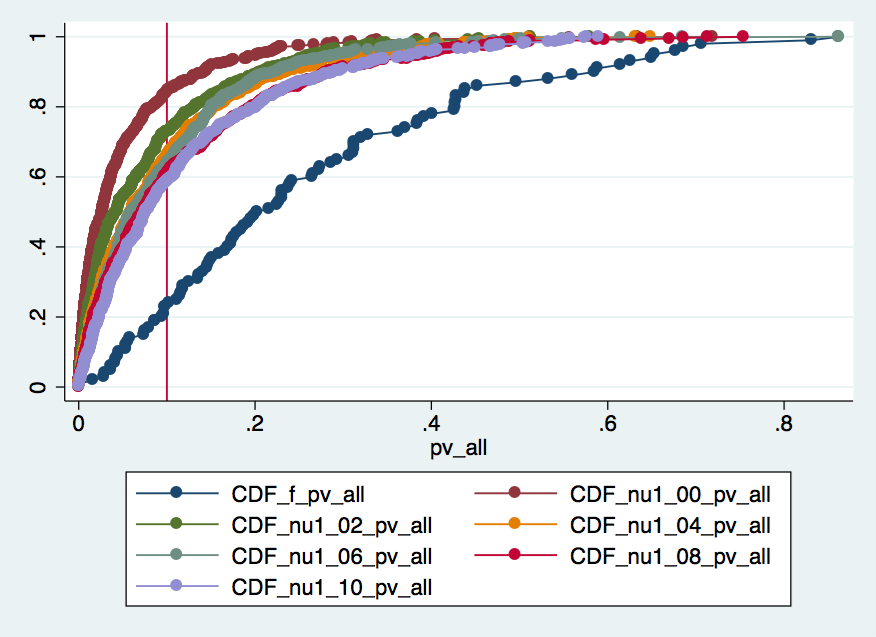
\includegraphics[width=.9\linewidth]{CDF_pva_nu1.png}\label{fig:CDFnu1}
	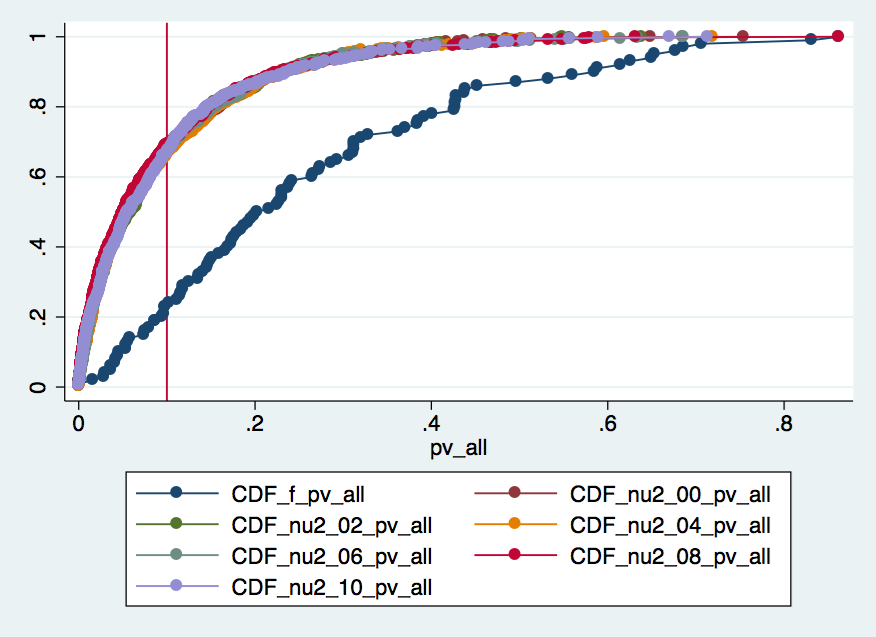
\includegraphics[width=.9\linewidth]{CDF_pva_nu2.png}\label{fig:CDFnu2}
  %\subfloat[][]{}
  %\subfloat[][]{}
  \caption{Cumulate Density Functions of p-values returned by goodness-of-fit tests to the (best-fit) power-law models for in-degree distributions of the interaction networks in the control and treatment groups. 20\% of the networks evolved without onboarding (dark blue) have degree distributions that test negatively for H1. When onboarding is introduced, that percentage rises to between 50 and 90\%. Above, the treatment group interaction networks have been grouped according to the value taken by $\nu_1$; below, they have been grouped according to the value taken by $\nu_2$ } 
 \label{fig:CDFpvanu1nu2}
\end{figure}

Onboarding effectiveness $\nu_1$ and community responsiveness $\nu_2$ seem to affect the in-degree distributions in different ways. Increasing $\nu_1$ pushes average p-values of the goodness-of-fit tests down, making it less likely that Hypothesis 1 would be rejected. Increasing $\nu_2$ seems not to play any role at all. This is somewhat surprising; higher values of $\nu_2$ lead to allocating an extra edge to the newcomer, and we have seen that allocating the first one (which is what happens when onboarding is introduced) has a strong negative effect on the p-value returned by the goodness-of-fit test. 

Regression analysis confirms the intuition from Figure \ref{fig:CDFpvanu1nu2}. We generated 6 dummy variables, each taking value 1 when $\nu_1 =  c$ and 0 otherwise, with $c = [0, 0.2, 0-4, 0-6, 0.8, 1]]$; next we generated 6 more dummy variables for the same vaules of $\nu_2$ . We then estimated a linear regression model with the p-value of our goodness-of-fit test as the dependent variable and the 12 dummy variables as its predictors. The results are:

\begin{enumerate}
\item Coefficients on predictors corresponding to different values of $\nu_1$ are positive and significant at the 0.05 level or better, with the exception of that corresponding to $\nu_1 = 0.2$.
\item Coefficients on predictors corresponding to different values of $\nu_2$ are non-significant.
\item Coefficients on interaction terms between $\nu_1$ and $\nu_2$ are non-significant.
\item A F-test of joint significance of the group of predictors corresponding to different values of $\nu_1$ strongly rejects the null hypothesis of non-significance (p-value: 0.0000).
\item A F-test of joint significance of the group of predictors corresponding to different values of $\nu_2$ does not reject the null hypothesis of non-significance (p-value: 0.9623).
\item A F-test of joint significance of the interaction terms does not reject the null hypothesis of non-significance (p-value: 0.1553).
\end{enumerate}

Full regression results are available in the appendix.

When we consider only the upper tail of the in-degree distribution (formula), the effect of introducing onboarding on the goodness-of-fit is much less clear. All but 32 (out of 3600) networks in the treatment group give rise to in-degree distributions that turn out to be a good fit for a power-law model when $k_{min}$ is chosen so as to minimize the Kolmogorov-Smirnov distance between the degree distributions themselves and their best-fit power-law models. We conclude that we do not reject Hypothesis 2, regardless of whether onboarding is present or not. This is illustrated by Table \ref{table:rejectsNoOb}

\begin{table}[h]
\centering
\caption{Number of rejects (out of 100 runs) for goodness-of-fit tests of power-law models to in-degree distributions of interaction networks in online communities, with no onboarding (control group) and with onboarding. Power-law models are estimated over all nodes with degree $k>=k_{min}$}
\label{table:rejectsNoOb}
\begin{tabular}{lllllll}
\hline
\multicolumn{7}{c} {Control group: 0}\\
\hline
  & nu2 = 0.0 & nu2 = 0.2 & nu2 = 0.4 & nu2 = 0.6 & nu2 = 0.8 & nu2 = 1\\
nu1 = 0.0        & 1        & 1        & 0        & 0        & 3        & 1      \\
nu1 = 0.2          & 1        & 0        & 1        & 3        & 1        & 1      \\
nu1 = 0.4          & 1        & 1        & 0        & 2        & 2        & 0      \\
nu1 = 0.6          & 0        & 0        & 2        & 1        & 1        & 0      \\
nu1 = 0.8          & 1        & 1        & 1        & 3        & 1        & 1      \\
nu1 = 1            & 0        & 0        & 1        & 0        & 0        & 0   \\
\hline  
\end{tabular}
\end{table}


\subsection{Lower bounds} \label {ssec:lower bounds}

Our results show a limited, albeit statistically significant, effect of onboarding on the value of formula, the value of formula that minimizes the Kolmogorov-Smirnov distance between the data generated by the computer simulation and the best-fit power-law model. Table \ref {table:ttestkMin} illustrates, for each value of  $\nu_1$ and $\nu_2$, the average value of $k_{min}$, and the result (expressed in p-value) of a t-test on the null hypothesis that such average value is the same as the corresponding statistics in the control group, against the alternative hypothesis that the former is greater than the latter. 

\begin{table}[h]
\centering
\caption{Average values of $k_{min}$ in the control group and in the treatment group by values of $\nu_1$ and $\nu_2$. The number in parenthesis is the p-value associated to a t-test that  $k_{min}(treatment) = k_{min}(control)$. }
\label{table:ttestkMin}
\begin{tabular}{lllllll}
\hline
\multicolumn{7}{c} {Control group: 3.43}\\
\hline
  & nu2 = 0.0 & nu2 = 0.2 & nu2 = 0.4 & nu2 = 0.6 & nu2 = 0.8 & nu2 = 1\\
nu1 = 0.0        & 3.88 (0.003)        & 3.91 (0.002)         & 3.87 (0.003)        & 3.74 (0.035)        & 3.87 (0.001)        & 3.98 (0.000)      \\
nu1 = 0.2          & 3.95 (0.000)        & 3.92 (0.001)        & 4.06 (0.000)        & 3.94 (0.001)        & 3.84 (0.004)        & 3.99 (0.001)      \\
nu1 = 0.4          & 4.2 (0.000)        & 4.11 (0.000)        & 4.14 (0.000)        & 3.91 (0.001)        & 4.04 (0.000)        & 4.21 (0.000)      \\
nu1 = 0.6          & 4.31 (0.000)        & 4.17 (0.000)        & 4.14 (0.000)        & 4.22 (0.000)        & 4.2 (0.000)        & 3.96 (0.000)      \\
nu1 = 0.8          & 4.23 (0.000)        & 4.55 (0.000)        & 4.22 (0.000)        & 4.14 (0.000)        & 4.17 (0.000)        & 4.27 (0.000)      \\
nu1 = 1            & 4.16 (0.000)         & 4.58 (0.000)        & 4.49 (0.000)        & 4.35 (0.000)        & 4.39 (0.000)        & 4.24 (0.000)   \\
\hline  
\end{tabular}
\end{table}

\begin{figure}[thb]
\centering

	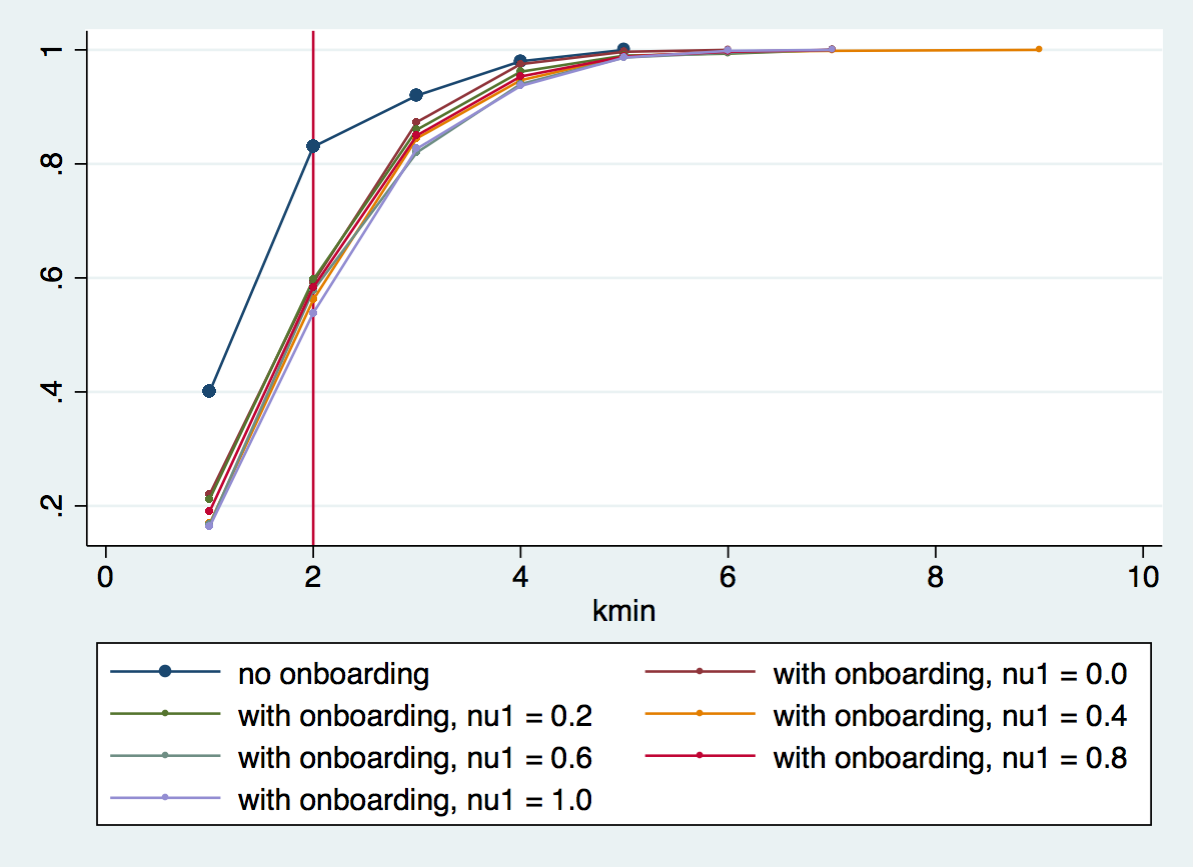
\includegraphics[width=.9\linewidth]{CDF_kmin_nu1.png}
	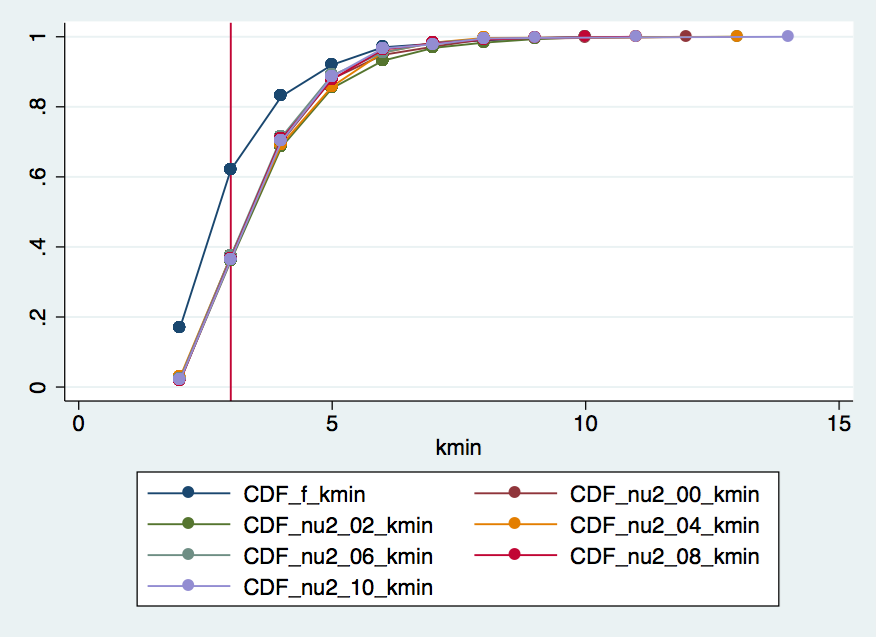
\includegraphics[width=.9\linewidth]{CDF_kmin_nu2.png}
  %\subfloat[][]{}
  %\subfloat[][]{}
  \caption{Cumulate Density Functions of the average value of $k_{min}$ that minimizes the Kolmogorov-Smirnov distance between the in-degree distribution of each interaction network and its best-fit power-law model.  returned by goodness-of-fit tests to the (best-fit) power-law models for in-degree distributions of the interaction networks in the control and treatment groups. 20\% of the networks evolved without onboarding (dark blue) have degree distributions that test negatively for H1. When onboarding is introduced, that percentage rises to between 50 and 90\%. Above, the treatment group interaction networks have been grouped according to the value taken by $\nu_1$; below, they have been grouped according to the value taken by $\nu_2$.} 
 \label{fig:CDFkminnu1nu2}
\end{figure}



A glance at figure \ref{fig:CDFkminnu1nu2} shows that over 60\% of the in-degree distributions from interaction networks in the control group, vis-a-vis only 30 to 40\% of those in the treatment group, fit a power-law model best for $k_{min}<=3$. Within the treatment group, some variability is associated to the increase of $\nu1$, whereas $\nu_2$ does not seem to play a significant role. Regression analysis, however, shows that, once we control for the presence of onboarding, neither parameter is significant. To prove this, we proceed analogously to section \ref{ssec:GOF of power law}: we estimated a linear regression model with the value of $k_{min}$ as the dependent variable and the 12 dummy variables as its predictors. The results are:

\begin{enumerate}
\item Coefficients on predictors corresponding to different values of $\nu_1$ are positive but non-significant, with the exception of that corresponding to $\nu_1 = 0.4$.
\item Coefficients on predictors corresponding to different values of $\nu_2$ are non-significant.
\item Coefficients on interaction terms between $\nu_1$ and $\nu_2$ are non-significant.
\item A F-test of joint significance of the group of predictors corresponding to different values of $\nu_1$ does not reject the null hypothesis of non-significance (p-value: 0.1227).
\item A F-test of joint significance of the group of predictors corresponding to different values of $\nu_2$ does not reject the null hypothesis of non-significance (p-value: 0.8682).
\item A F-test of joint significance of the interaction terms does not reject the null hypothesis of non-significance (p-value: 0.7456).
\end{enumerate}

Full regression analysis is available in the appendix.


\subsection{Exponents} \label{ssec:exponents}
We find that introducing onboarding to an online community has a positive and significant on the value of the exponent of the best-fit power-law model for the in-degree distribution of its interaction network. This is consistent with the theoretical results by Dorogovtsev and Mendes \cite{dorogovtsev2002evolution}, who proved that introducing a fraction of non-preferential attachment edges in evolving networks with preferential attachment does not suppress the power-law dependence of its degree distribution, but only increases the scaling exponent thereof. 

This result holds when the best-fit power-law models is computed over $k>=k_{min}$, where $k_{min}$ is, as usual, the value of $k$ that minimizes the Kolmogorov-Smirnov distance between the simulated in-degree distribution and its best-fit power-law model. When it is computed over the whole support of the in-degree distribution ($k>= 1$), it also holds, except for $\nu_1 = 1$; in the latter case, the null hypothesis that the values of the exponent in the control and in the treatment groups are drawn from the same distribution cannot be rejected. Tables \ref {table:ttestExpA} and \ref {table:ttestExp} illustrate, for each value of  $\nu_1$ and $|nu_2$, the average value of the scaling parameter $\alpha$, and the result (expressed in p-value) of a t-test on the null hypothesis that such average value is the same as the corresponding statistics in the control group, against the alternative hypothesis that the former is greater than the latter. Table \ref{table:ttestExpA} refers to $k>= 1$, whereas Table \ref{table:ttestExp} refers to $k_{min}$.

\begin{table}[h]
\centering
\caption{Average values of the power-law model's exponent $\alpha$ in the control group and in the treatment group by values of $\nu_1$ and $\nu_2$, computed over the whole support $k>=1$. The number in parenthesis is the p-value associated to a t-test that  $\alpha(treatment) = \alpha(control)$. }
\label{table:ttestExpA}
\begin{tabular}{lllllll}
\hline
\multicolumn{7}{c} {Control group: 1.752}\\
\hline
  & nu2 = 0.0 & nu2 = 0.2 & nu2 = 0.4 & nu2 = 0.6 & nu2 = 0.8 & nu2 = 1\\
nu1 = 0.0        & 1.889 (0.000)        & 1.888 (0.000)         & 1.888 (0.000)        & 1.887 (0.000)        & 1.887 (0.000)        & 1.888 (0.000)      \\
nu1 = 0.2          & 1.848 (0.000)        & 1.849 (0.000)        & 1.848 (0.000)        & 1.849 (0.000)        & 1.849 (0.000)        & 1.849 (0.000)      \\
nu1 = 0.4          & 1.818 (0.000)        & 1.818 (0.000)        & 1.817 (0.000)        & 1.817 (0.000)        & 1.817 (0.000)        & 1.819 (0.000)      \\
nu1 = 0.6          & 1.792 (0.000)        & 1.792 (0.000)        & 1.792 (0.000)        &  1.792 (0.000)        & 1.792 (0.000)        & 1.792 (0.000)      \\
nu1 = 0.8          & 1.771 (0.000)        & 1.771 (0.000)        & 1.771 (0.000)        & 1.771 (0.000)        & 1.771 (0.000)        & 1.772 (0.000)      \\
nu1 = 1            & 1.753 (0.211)         & 1.753 (0.202)        & 1.753 (0.263)        & 1.753 (0.430)        & 1.753 (0.239)        & 1.753 (0.191)   \\
\hline  
\end{tabular}
\end{table}

\begin{table}[h]
\centering
\caption{Average values of the power-law model's exponent $\alpha$ in the control group and in the treatment group by values of $\nu_1$ and $\nu_2$, computed over$k>=k_{min}$. We omit the p-values associated to a t-test that  $\alpha_{treatment} = \alpha_{control}$, as they are smaller than 0.001 in all cases. }
\label{table:ttestExp}
\begin{tabular}{lllllll}
\hline
\multicolumn{7}{c} {Control group: 2.419}\\
\hline
 & nu2 = 0.0 & nu2 = 0.2 & nu2 = 0.4 & nu2 = 0.6 & nu2 = 0.8 & nu2 = 1\\
nu1 = 0.0        & 2.985        & 2.989        & 2.868    & 3.000    & 3.004        & 3.015       \\
nu1 = 0.2          & 2.855        & 2.852        & 2.868        & 2.834        & 2.821        & 2.854      \\
nu1 = 0.4          & 2.746        & 2.727        & 2.735        & 2.725        & 2.739        & 2.749      \\
nu1 = 0.6          & 2.661        & 2.655        & 2.632        & 2.650        & 2.656        & 2.623      \\
nu1 = 0.8          & 2.562        & 2.602        & 2.571        & 2.553    & 2.554        & 2.553      \\
nu1 = 1            & 2.496        & 2.527        & 2.518        & 2.514        & 2.514        & 2.499   \\
\hline  
\end{tabular}
\end{table}

We inspect further the impact of parameters $\nu_1$ and $\nu_2$ via regression analysis. It shows that the former has a significant impact, whereas the latter does not. To prove this, we proceed analogously to section \ref{ssec:GOF of power law}: we estimate two linear regression models with the 12 dummy variables as its predictors. In the first one, the dependent variable is the value of the power-law model's exponent $\alpha$ when the model is estimated over the whole support of the in-degree distribution for each interaction network. In the second one, the dependent variable is power-law model's exponent $\alpha$ when the model is estimated over $k>=k_{min}$. The results for both models are very similar:

\begin{enumerate}
\item Coefficients on predictors corresponding to different values of $\nu_1$ are negative and highly significant, though small.
\item Coefficients on predictors corresponding to different values of $\nu_2$ are non-significant.
\item Coefficients on interaction terms between $\nu_1$ and $\nu_2$ are non-significant.
\item A F-test of joint significance of the group of predictors corresponding to different values of $\nu_1$ rejects the null hypothesis of non-significance (p-values: 0.000 for both models). 
\item A F-test of joint significance of the group of predictors corresponding to different values of $\nu_2$ does not reject the null hypothesis of non-significance (p-values:  0.4425 for $k >= 1$,  0.4034 for $k>= k_{min}$).
\item A F-test of joint significance of the interaction terms does not reject the null hypothesis of non-significance (p-values:  0.9177 for $k >= 1$,  0.8271 for $k>= k_{min}$)  .
\end{enumerate}.

Full regression analysis is available in the appendix.

